\chapter{Results}\label{chap:results}

\section{Total energy as a function of time for different time steps}
    \graphicspath{ {./figures/milestone04/} }
    \begin{figure}[!htb]
    % \captionsetup{justification=centering,margin=2cm}
    \centering
        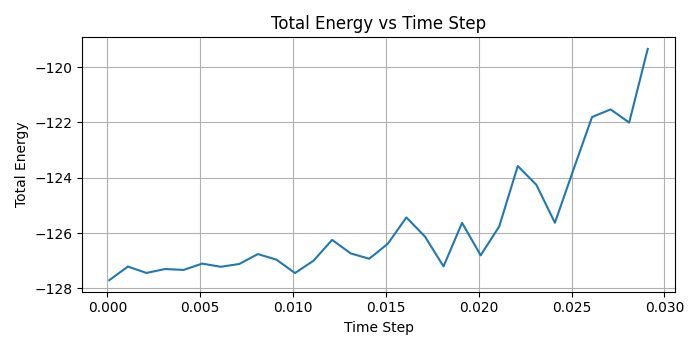
\includegraphics[scale=0.9]{total_energy_vs_time_step.png}
        \caption[Total energy vs Time steps using parameters]{\textbf{Total energy vs Time steps using parameters: start\_time\_step=1e-4, end\_time\_step=30e-3,step=1e-3, sigma=1, mass=1, epsilon=1, total\_time=5000}}
    \label{fig:total_energy_vs_time_step}
    \end{figure}


\section{Snapshots sequence of LJ simulation}
    \graphicspath{ {./figures/milestone04/} }
    \begin{figure}[h]

    \centering
        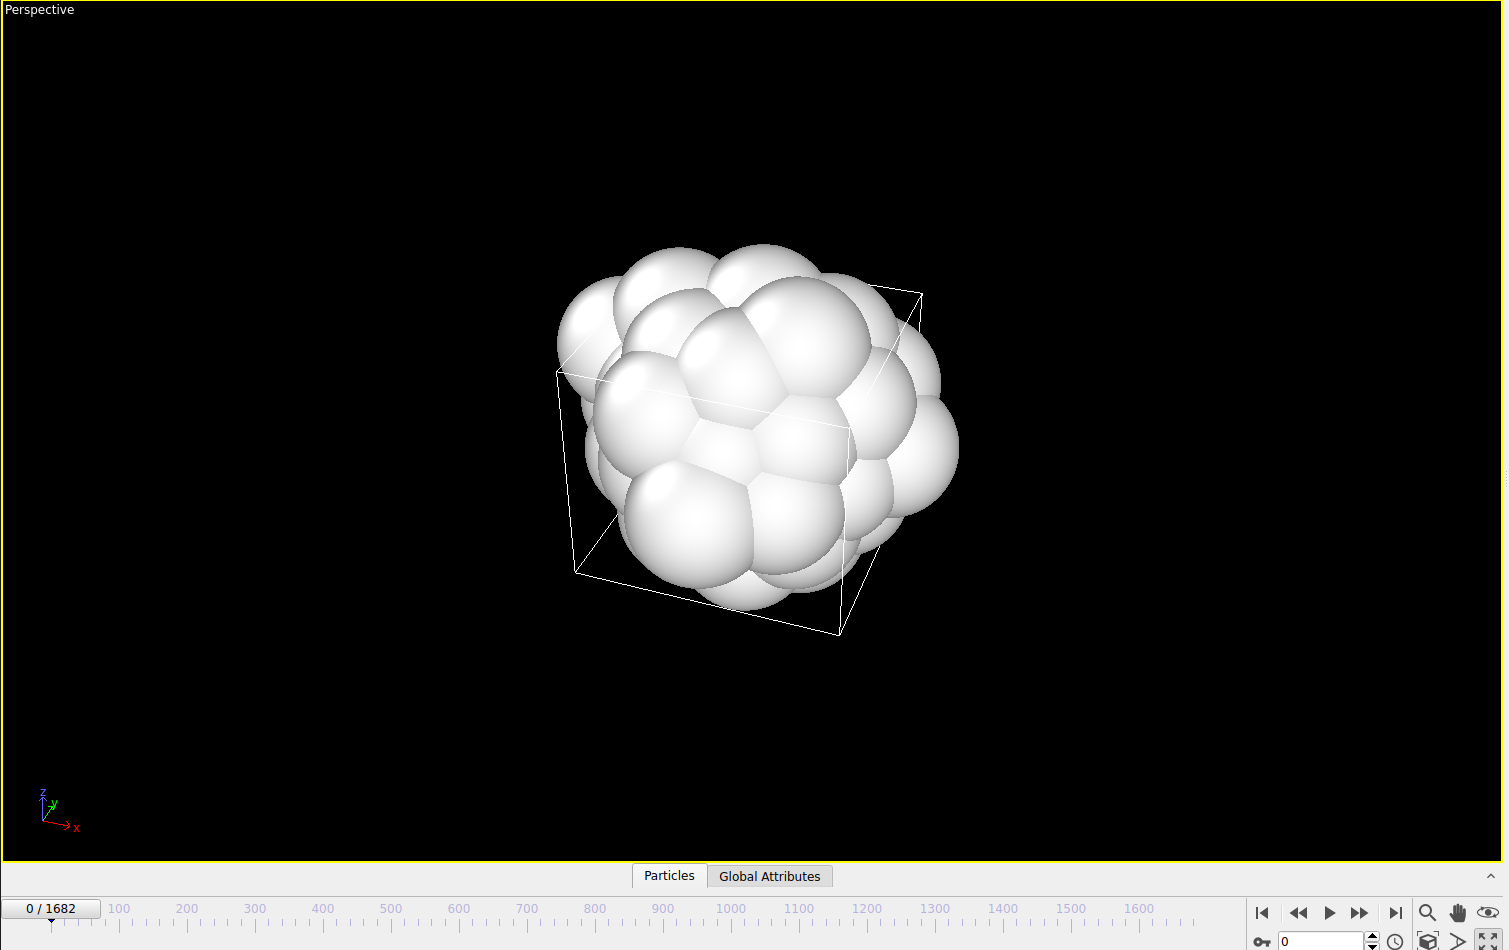
\includegraphics[scale=0.25]{ML1.png}
        \caption{LJ simulation snapshot1}
    \label{fig:step1}
    \end{figure}
    \begin{figure}[!htb]
    \centering
        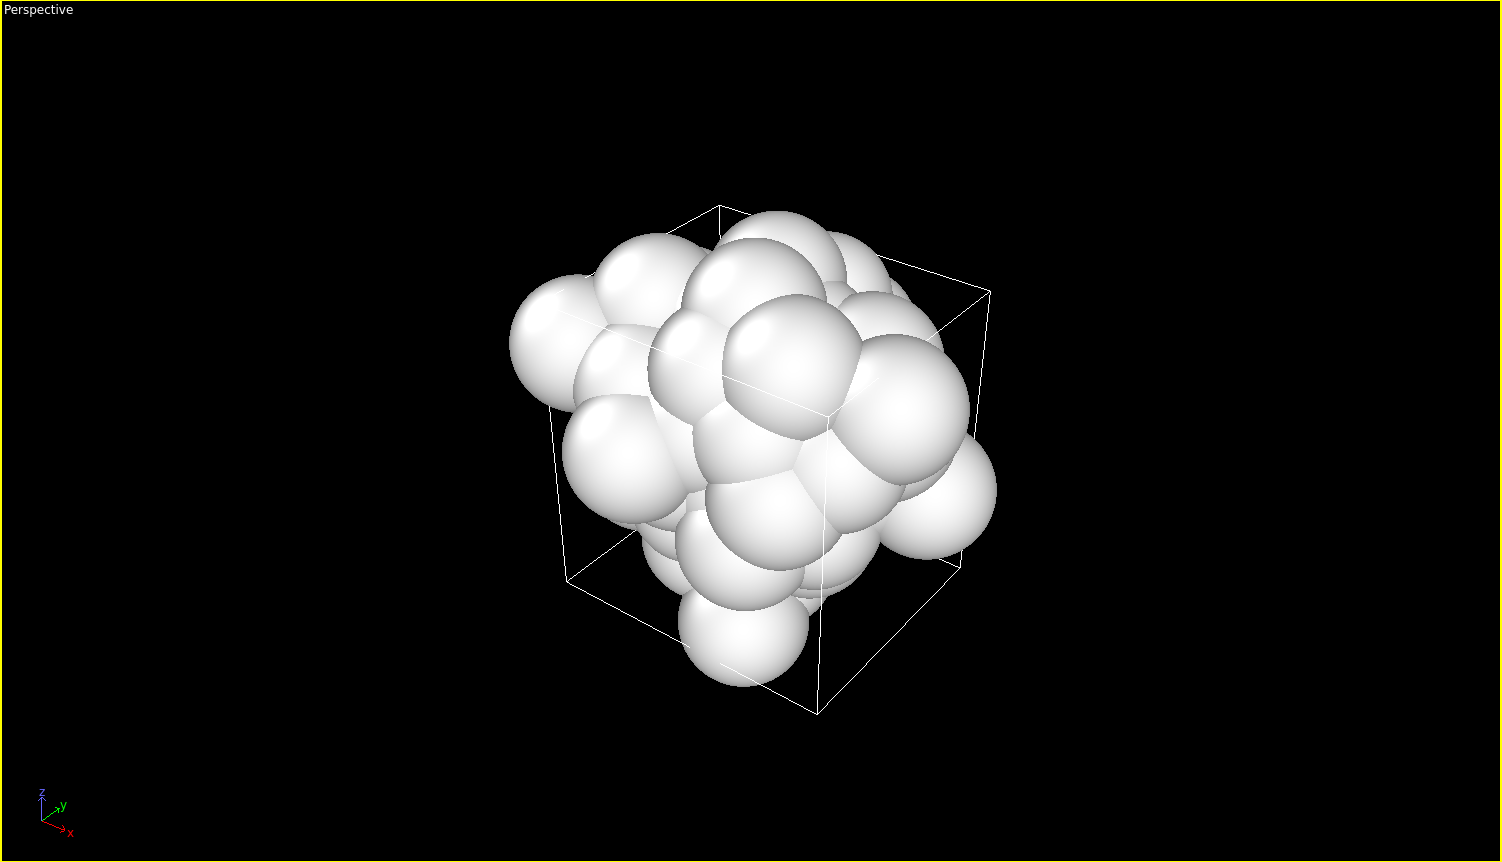
\includegraphics[scale=0.25]{ML2.png}
        \caption{LJ simulation snapshot2}
    \label{fig:step2}
    \end{figure}
    \begin{figure}[!htb]
    \centering
        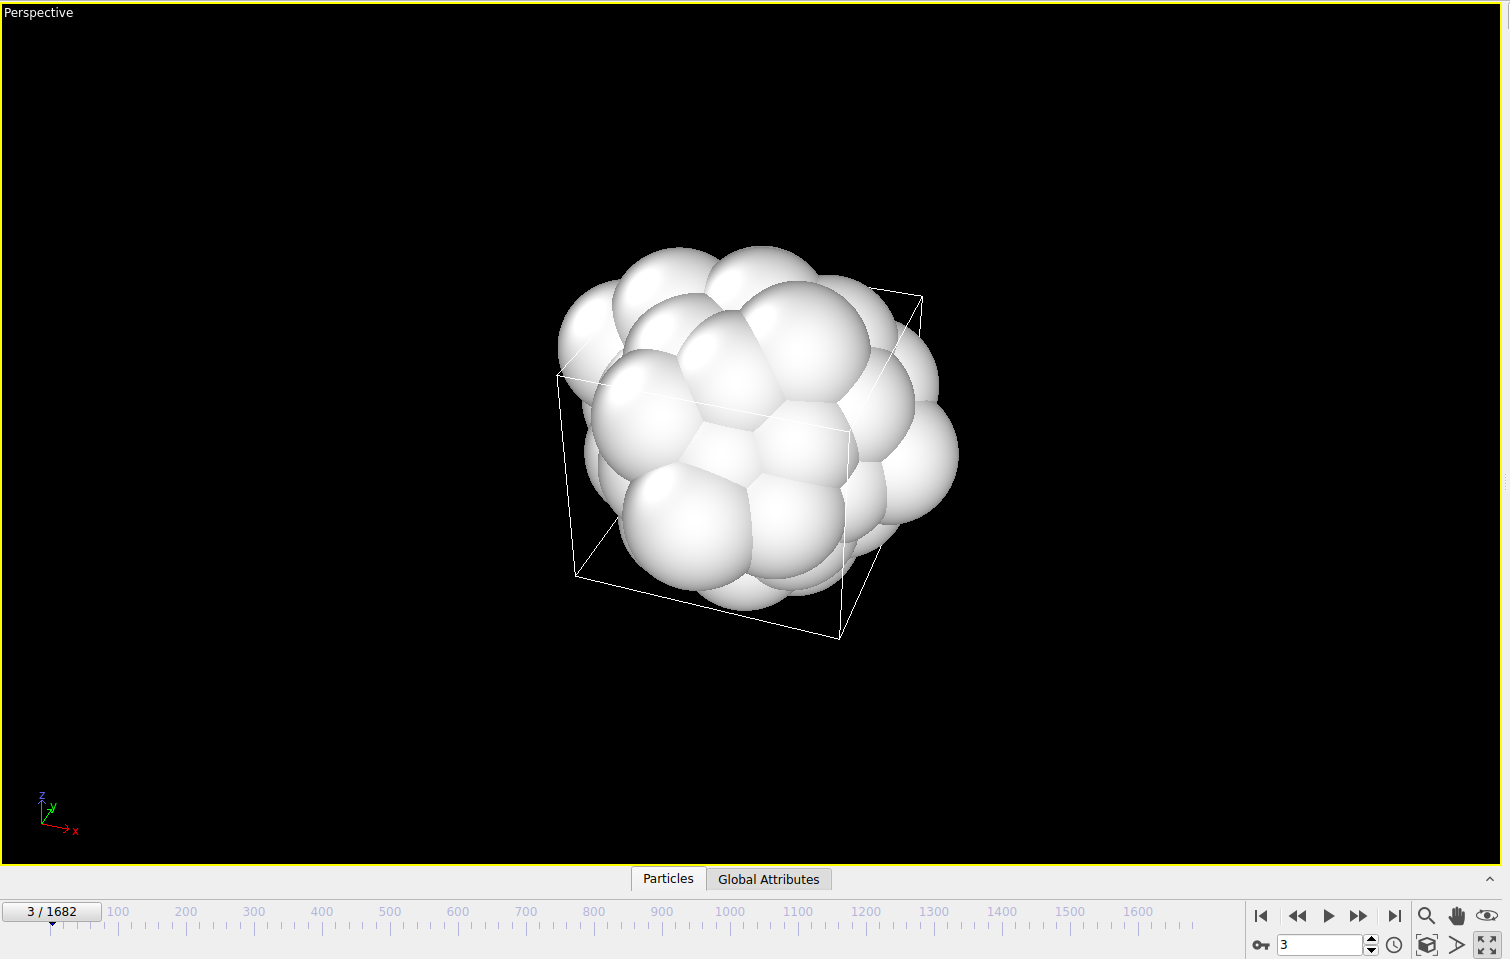
\includegraphics[scale=0.25]{ML3.png}
        \caption{LJ simulation snapshot3}
    \label{fig:step3}
    \end{figure}
    \begin{figure}[!htb]
    \centering
        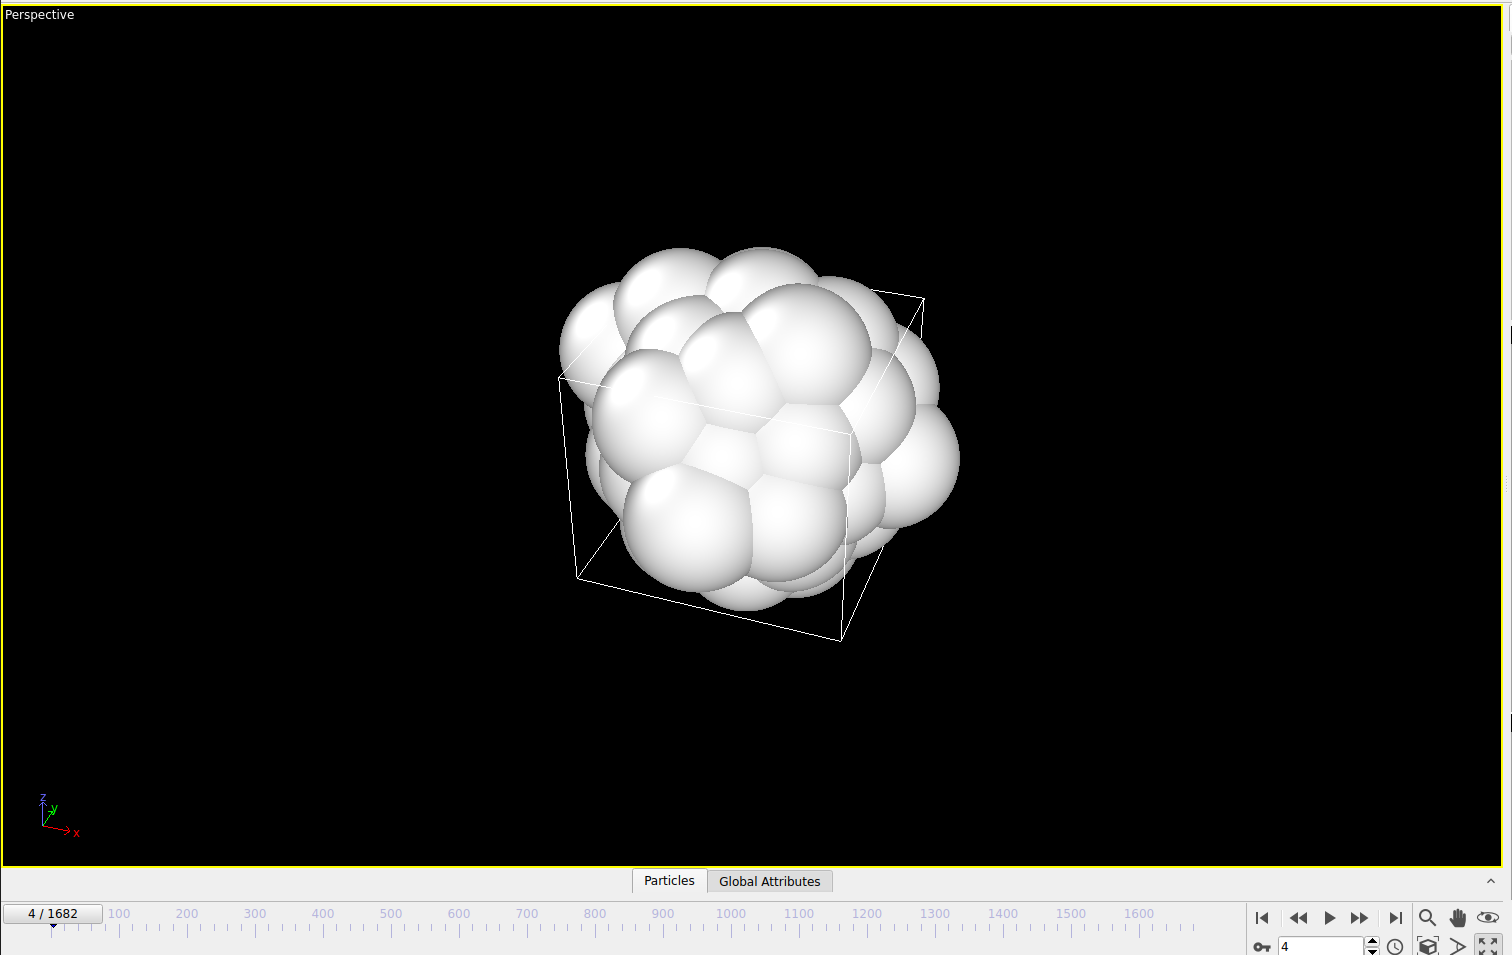
\includegraphics[scale=0.25]{ML4.png}
        \caption{LJ simulation snapshot4}
    \label{fig:step4}
    \end{figure}
    \begin{figure}[!htb]
    \centering
        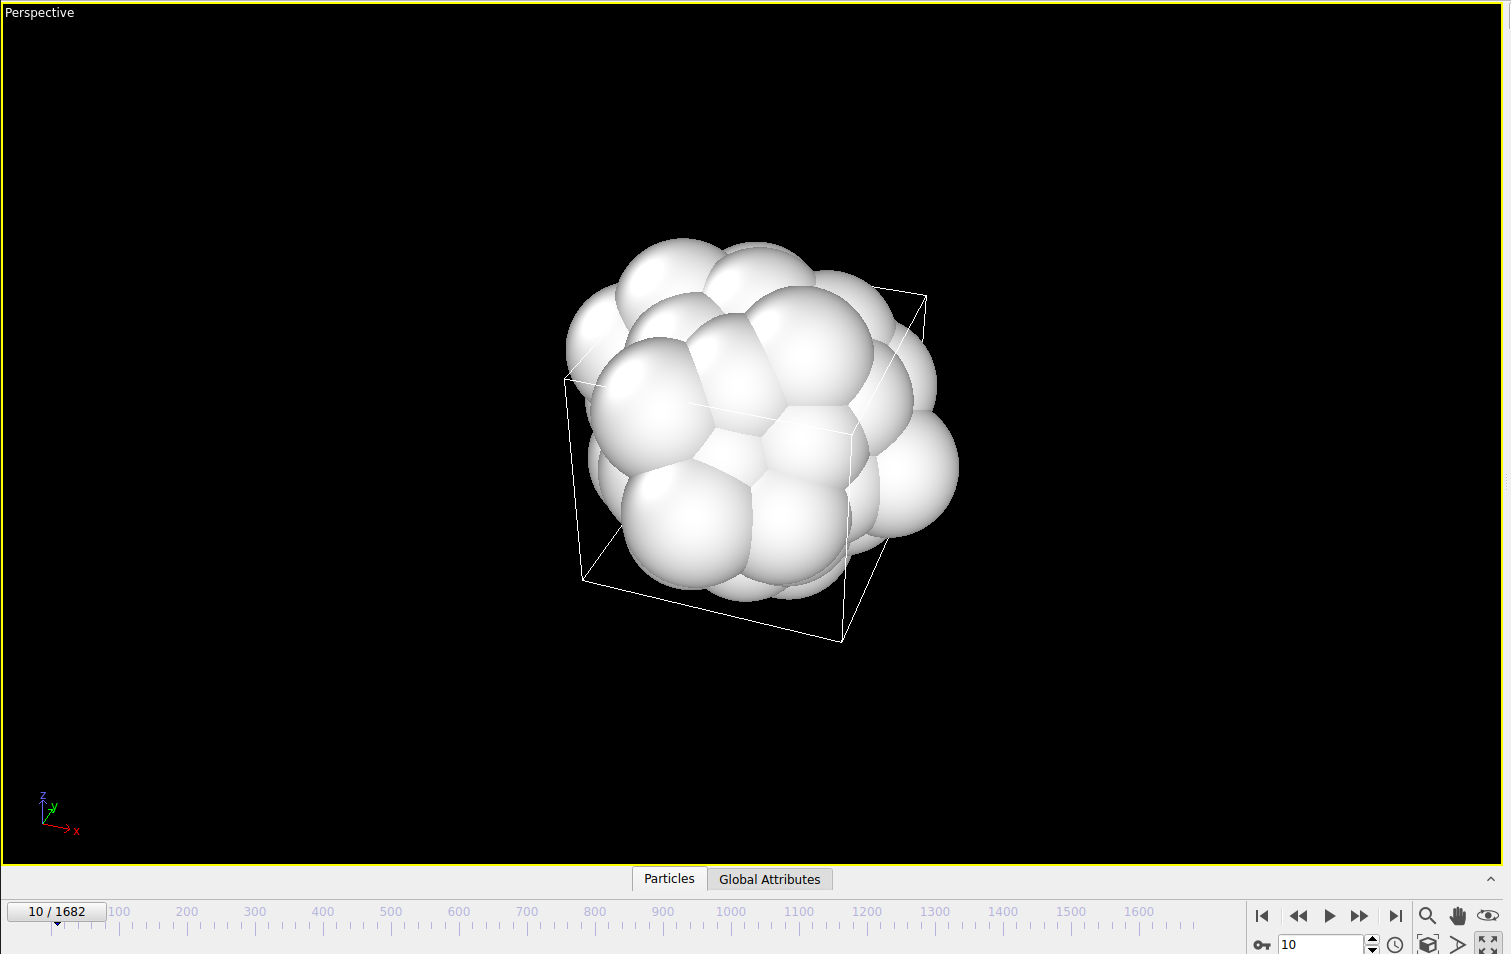
\includegraphics[scale=0.25]{ML5.png}
        \caption{LJ simulation snapshot5}
    \label{fig:step5}
    \end{figure}



\section{simulation time as a function of the size (number of atoms) without neighbor list}
\graphicspath{ {./figures/milestone05/} }
\begin{figure}[!htb]
\centering
    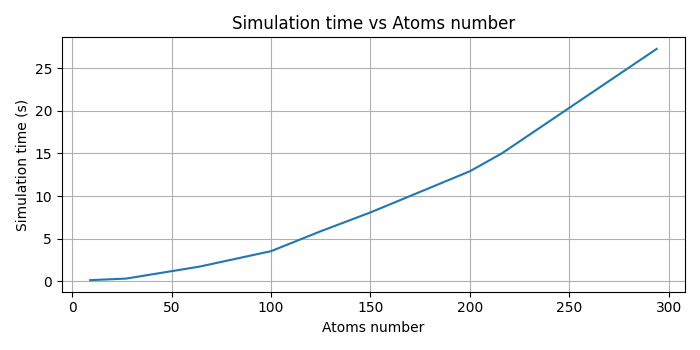
\includegraphics[scale=0.9]{simulation_time_vs_atoms_number.png}
    \caption[Simulation time vs Atoms number]{\textbf{caption[Simulation time vs Atoms number using parameters: time\_step=1e-3, sigma=1, mass=1, epsilon=1, total\_time=5000, relaxation\_time\_start = 10* time\_step,then after reaching equilibrium, it increases to 50*time\_step.}}
\label{fig:simulation_time_vs_atoms_number}
\end{figure}
Here we notice that the simulation time increases quadratically with the number of atoms in the system. This is because in the energy update step in the LJ simulation we have to calculate the energy between all the pairs of atoms in the system. So the time complexity of the energy update step is $O(N^2)$ where $N$ is the number of atoms in the system. For example, In the figure above,The  simulation time for 100 atoms is 3.5s and for 200 atoms is 12.9s which is almost 4 times more than the simulation time for 100 atoms.

\section{simulation time as a function of the size (number of atoms) with neighbor list}
\graphicspath{ {./figures/milestone06/} }
\begin{figure}[!htb]
\centering
    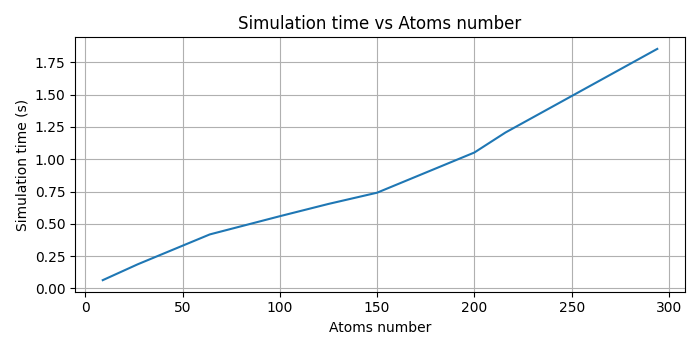
\includegraphics[scale=0.9]{simulation_time_vs_atoms_number.png}
    \caption[Simulation time vs Atoms number]{\textbf{caption[Simulation time vs Atoms number using parameters: time\_step=1e-3, sigma=1, mass=1, epsilon=1, total\_time=5000, relaxation\_time\_start = 10* time\_step,then after reaching equilibrium, it increases to 50*time\_step, and cutoff\_radius = 1.5.}}
\label{fig:simulation_time_vs_atoms_number}
\end{figure}
Here, it's very clear the linearity of the simulation time with the number of atoms in the system. By introducing the concept of just calculating the energy between the atoms that are close to each other, we have reduced the time complexity of the energy update step from $O(N^2)$ to $O(N)$ where $N$ is the number of atoms in the system. For example, In the figure above,The  simulation time for 100 atoms is 0.56s and for 200 atoms is 1.05s which is almost 2 times more than the simulation time for 100 atoms.

\section{total energy vs temperature}
\section{melting point versus cluster size}
\section{heat capacity versus cluster size}
\section{latent heat versus cluster size}
\section{Energy conservation with MPI parallelization}
% \section{Nanowire σ/ɛ}
\section{Nanowire defects}